\begin{frame}
  \frametitle{Reinforcement Learning}
  \begin{columns}
      \begin{column}{0.45\textwidth}
        \begin{itemize}
          \item{definition}
          \item{basic concepts:}
            \begin{itemize}
              \item{agent,}
              \item{environment,}
              \item{states,}
              \item{actions,}
              \item{rewards,}
              \item{etc.}
            \end{itemize}
          \item{machine learning branches:}
            \begin{itemize}
              \item{RL vs supervised learning,}
              \item{RL vs unsupervised}
            \end{itemize}
        \end{itemize}
      \end{column}

      \begin{column}{0.45\textwidth}
        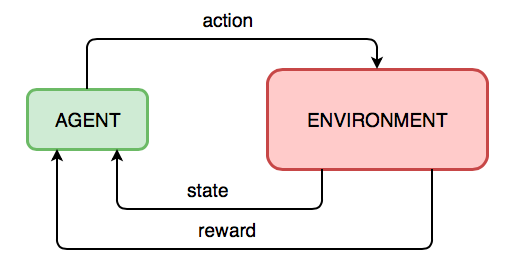
\includegraphics[width=\textwidth]{imgs/rl_model.png}
      \end{column}
  \end{columns}
\end{frame}
